\chapter{Implementacija i korisničko sučelje}
		
		\section{Korištene tehnologije i alati}
		
			\textbf{\textit{dio 2. revizije}}
			
			 \textit{Detaljno navesti sve tehnologije i alate koji su primijenjeni pri izradi dokumentacije i aplikacije. Ukratko ih opisati, te navesti njihovo značenje i mjesto primjene. Za svaki navedeni alat i tehnologiju je potrebno \textbf{navesti internet poveznicu} gdje se mogu preuzeti ili više saznati o njima}.
			
			
			\eject 
		
	
		\section{Ispitivanje programskog rješenja}
			
			\subsection{Ispitivanje komponenti}
			{Svi endpointovi na backend-u su ručno testirani, a ispitivanje jedinica (engl. unit testing) proveli smo nad osnovnim funkcionalnostima servisnog sloja koristeći biblioteku junit. Prilikom testiranja pojedinog razreda, servise i repozitorije čije metode taj razred poziva smo \textit{mock-ali} koristeći biblioteku mockito, pa smo samo u svakoj test metodi zadali što će pojedina pozvana metoda vraćati.}
			
			\textbf{1. UserServiceTests\\}
			{U UserServiceTests testnoj klasi ispitali smo funkcionalnost dodavanja novog korisnika u bazu podataka.\\
			Naredbom \textit{Mockito.when(userRepository.save(Mockito.any())).thenReturn(test);} smo rekli mockanom userRepository-ju kako da se ponaša prilikom poziva save metode.}
			\begin{figure}[H]
				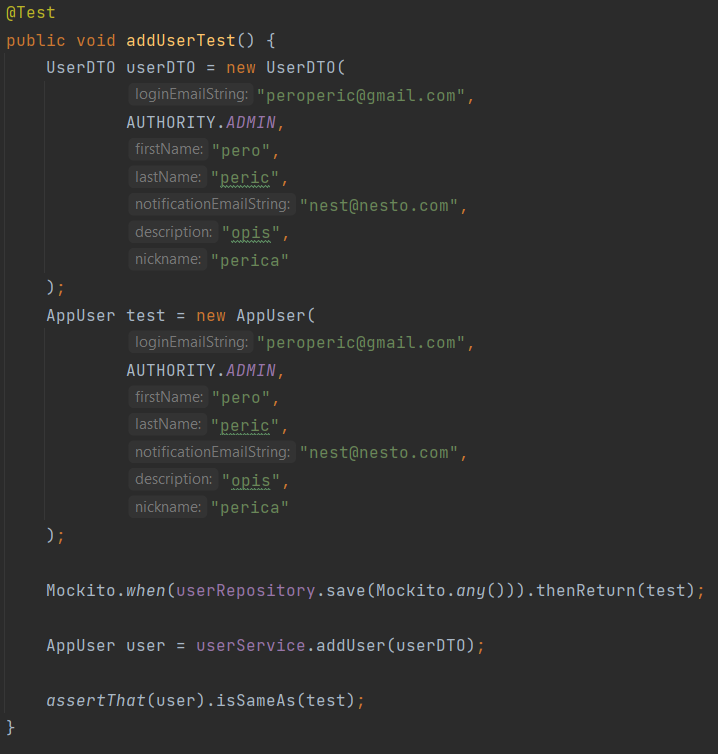
\includegraphics[scale=0.6]{UnitTests/addUserTest}
				\centering
				\caption{Add user test}
				\label{fig:addUserTest}
			\end{figure}
			\begin{figure}[H]
				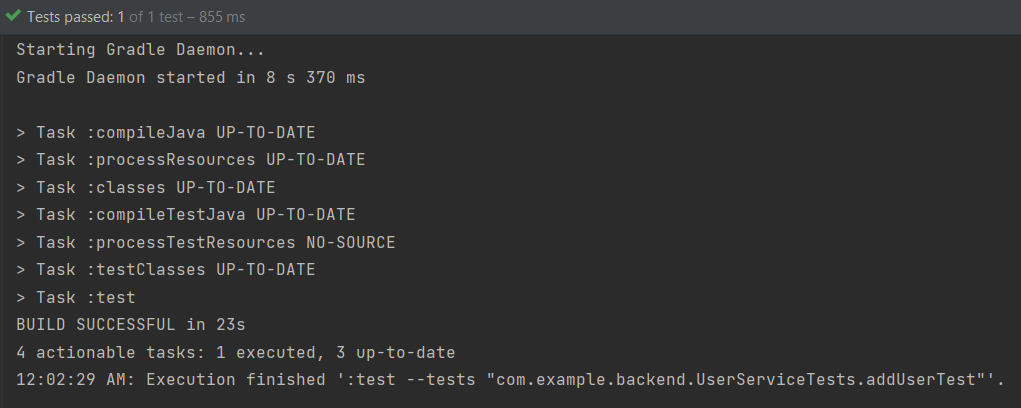
\includegraphics[scale=0.5]{UnitTests/addUserTestResult}
				\centering
				\caption{Add user test result}
				\label{fig:addUserTestResult}
			\end{figure}
			
			\textbf{2. ProjectServiceTests\\}
			{U ProjectServiceTests klasi smo ispitali funkcionalnosti dohvata projekta iz baze podataka te dodavanje FR team membera na projekt.}
			\begin{figure}[H]
				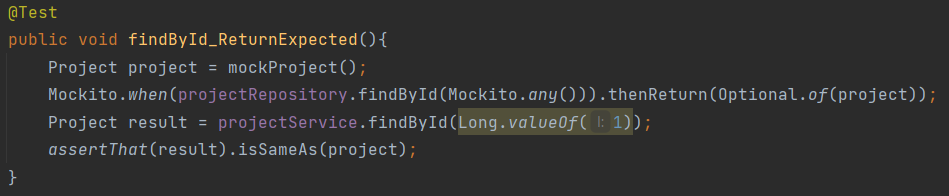
\includegraphics[scale=0.6]{UnitTests/projectFindById}
				\centering
				\caption{Find project by Id test}
				\label{fig:projectFindByIdTest}
			\end{figure}
			\begin{figure}[H]
				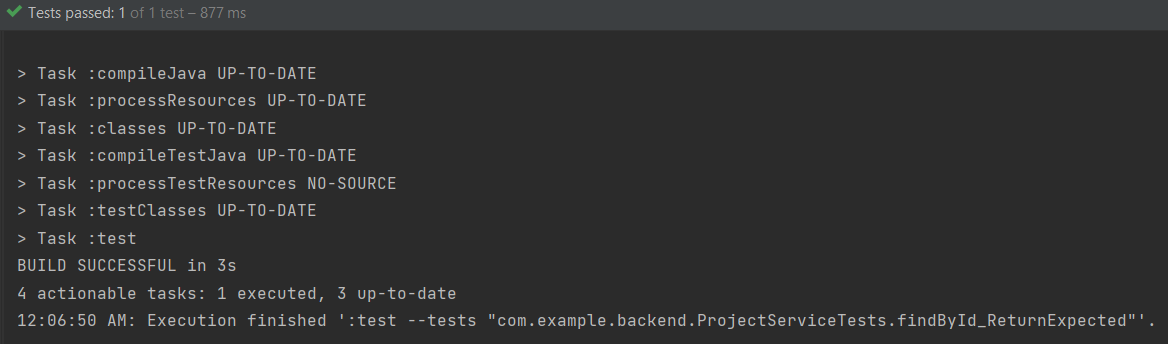
\includegraphics[scale=0.6]{UnitTests/projectFindByIdResult}
				\centering
				\caption{Find project by Id test result}
				\label{fig:projectFindByIdResult}
			\end{figure}

			\begin{figure}[H]
				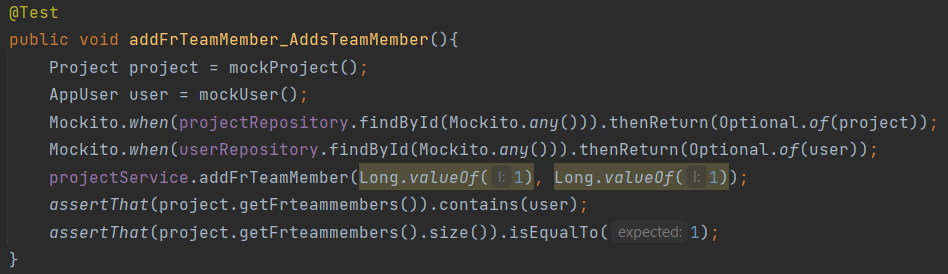
\includegraphics[scale=0.5]{UnitTests/projectAddFrTeamMember}
				\centering
				\caption{Add FR team member to project test}
				\label{fig:addFrTeamMemberTest}
			\end{figure}
			\begin{figure}[H]
				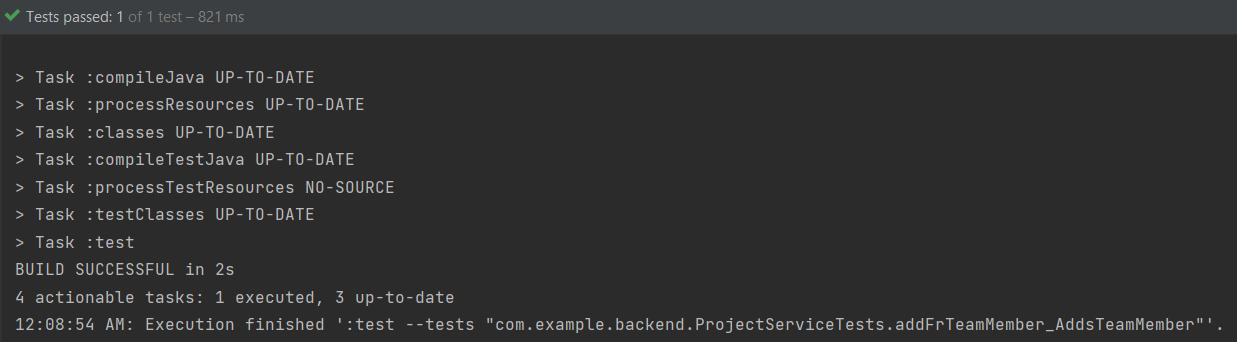
\includegraphics[scale=0.4]{UnitTests/projectAddFrTeamMemberResult}
				\centering
				\caption{Add FR team member result}
				\label{fig:addFrTeamMemberResult}
			\end{figure}

			\textbf{3. CompanyServiceTests\\}
			{U CompanyServiceTests klasi smo ispitali sljedeće funkcionalnosti:\\
				Kreiranje nove kompanije\\
				Dohvaćanje svih kompanij\\
				Bacanje EntityNotFoundException-a prilikom pokušaja brisanja nepostojeće kompanije\\
				Bacanje AuthenticationException-a prilikom pokušaja dohvata podataka od kompanije od strane Usera koji je samo Observer}
			
			\begin{figure}[H]
				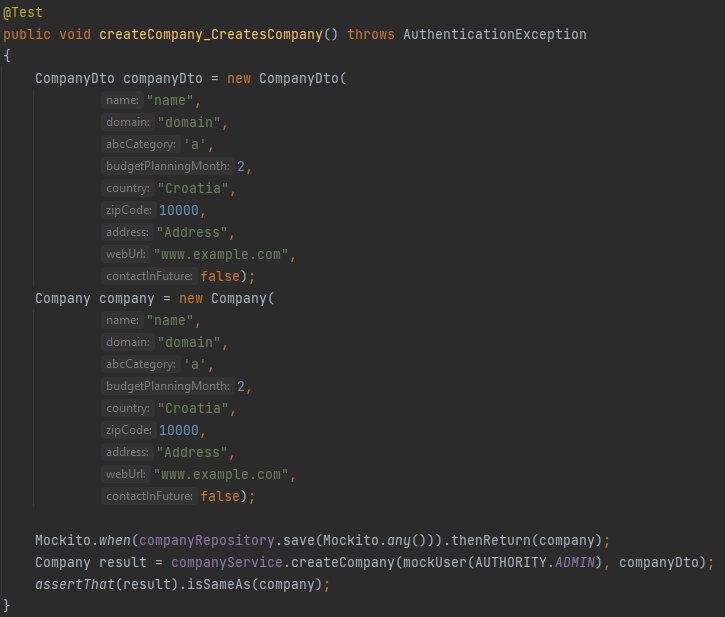
\includegraphics[scale=0.5]{UnitTests/createCompany}
				\centering
				\caption{Create company test}
				\label{fig:createCompanyTest}
			\end{figure}
			\begin{figure}[H]
				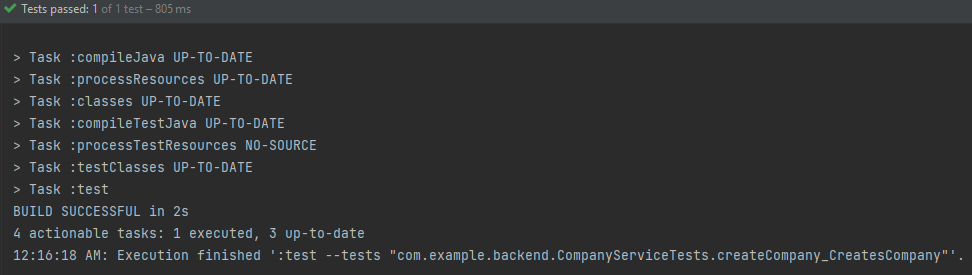
\includegraphics[scale=0.4]{UnitTests/createCompanyResult}
				\centering
				\caption{Create company test result}
				\label{fig:createCompanyResult}
			\end{figure}

			\begin{figure}[H]
				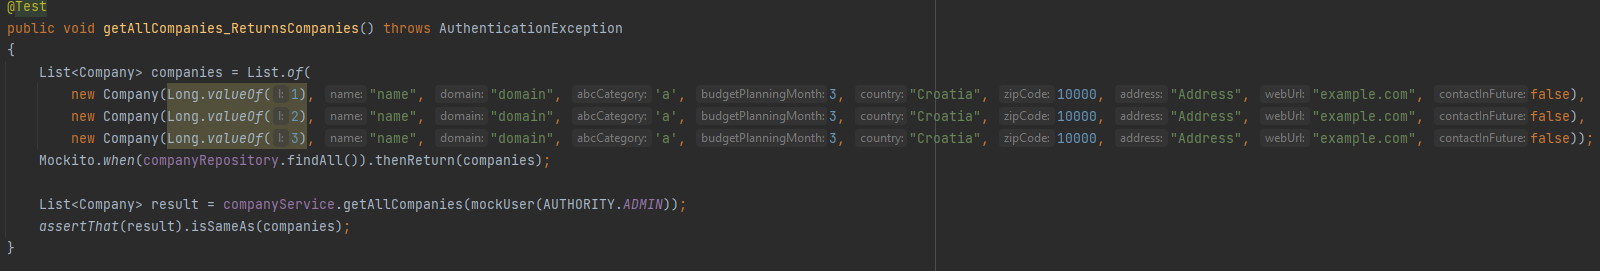
\includegraphics[scale=0.3]{UnitTests/getAllCompanies}
				\centering
				\caption{Get all companies test}
				\label{fig:getAllCompaniesTest}
			\end{figure}
			\begin{figure}[H]
				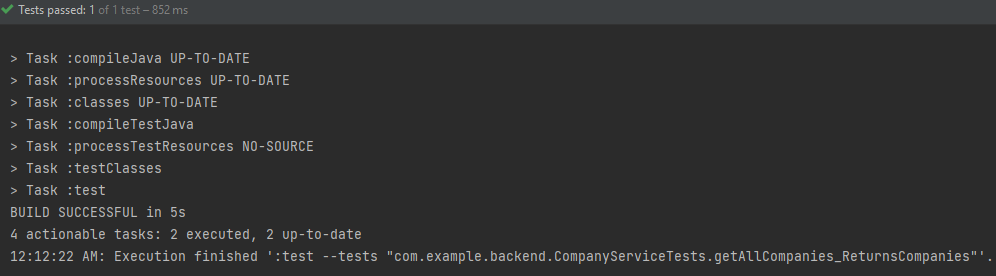
\includegraphics[scale=0.4]{UnitTests/getAllCompaniesResult}
				\centering
				\caption{Get all companies test result}
				\label{fig:getAllCompaniesResult}
			\end{figure}

			\begin{figure}[H]
				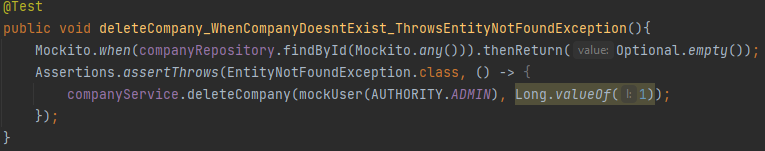
\includegraphics[scale=0.5]{UnitTests/deleteCompanDoesntExist}
				\centering
				\caption{Delete company which does not exist test}
				\label{fig:deleteCompanyTest}
			\end{figure}
			\begin{figure}[H]
				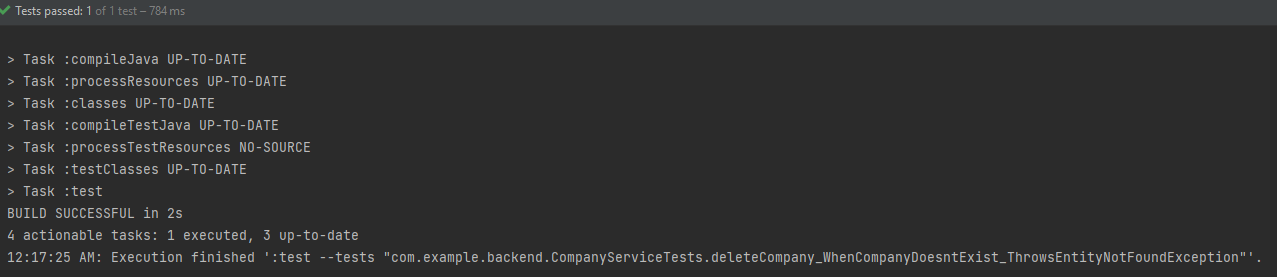
\includegraphics[scale=0.4]{UnitTests/deleteCompanDoesntExistResult}
				\centering
				\caption{Delete company which does not exist tes result}
				\label{fig:deleteCompanyResult}
			\end{figure}

			\begin{figure}[H]
				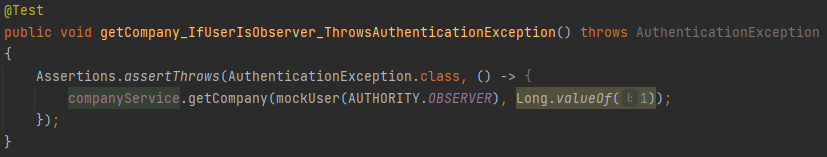
\includegraphics[scale=0.5]{UnitTests/getCompanyObserver}
				\centering
				\caption{Get company info by observer test}
				\label{fig:getCompanyObserver}
			\end{figure}
			\begin{figure}[H]
				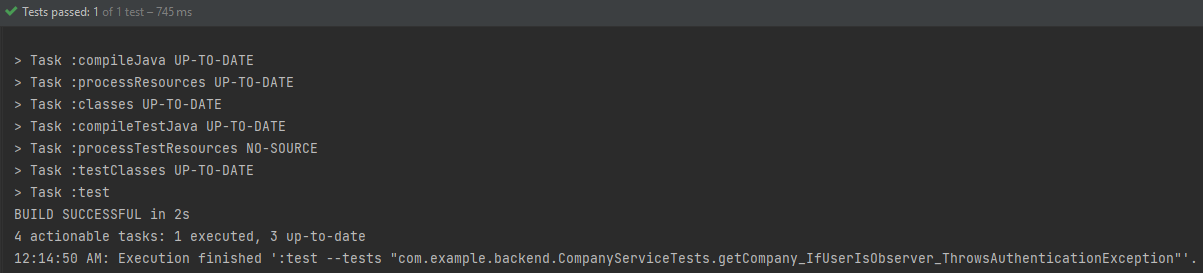
\includegraphics[scale=0.4]{UnitTests/getCompanyObserverResult}
				\centering
				\caption{Get company info by observer test result}
				\label{fig:getCompanyObserverResult}
			\end{figure}
			
			\textbf{4. CollaborationServiceTests\\}
			{U CollaborationServiceTests testnoj klasi smo ispitali funkcionalnost dodavanja suradnje u bazu podataka.}

			\begin{figure}[H]
				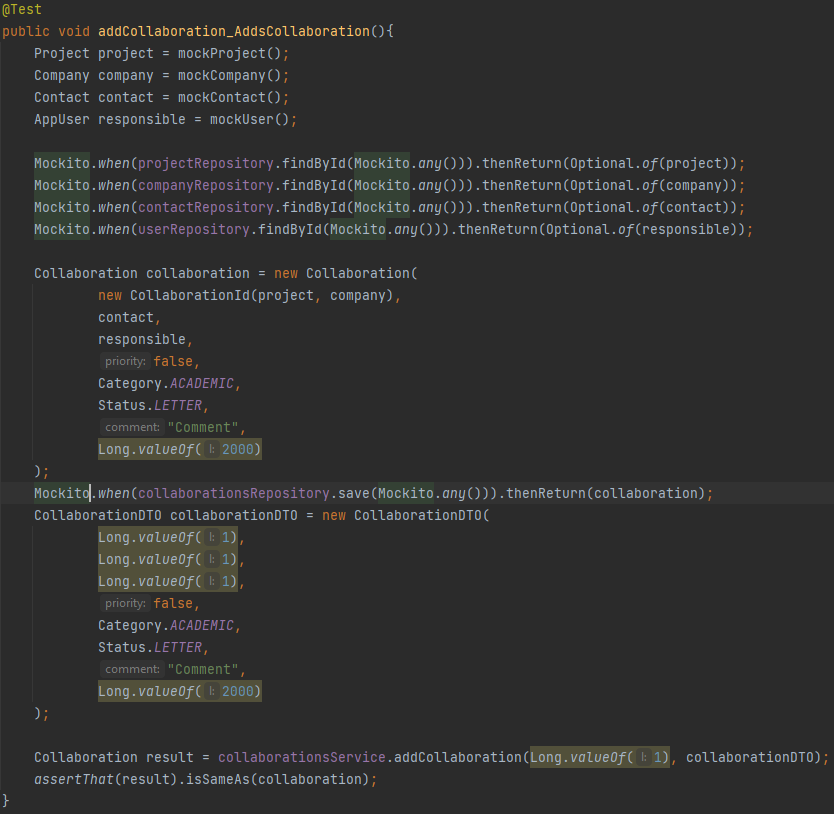
\includegraphics[scale=0.5]{UnitTests/addCollaboration}
				\centering
				\caption{Add collaboration test}
				\label{fig:addCollaboration}
			\end{figure}
			\begin{figure}[H]
				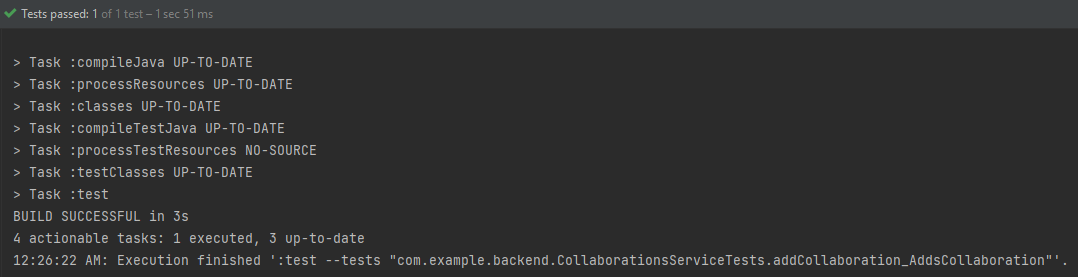
\includegraphics[scale=0.4]{UnitTests/addCollaborationResult}
				\centering
				\caption{Add collaboration test result}
				\label{fig:addCollaborationResult}
			\end{figure}

			\subsection{Ispitivanje sustava}
			
			 \textit{Potrebno je provesti i opisati ispitivanje sustava koristeći radni okvir Selenium\footnote{\url{https://www.seleniumhq.org/}}. Razraditi \textbf{minimalno 4 ispitna slučaja} u kojima će se ispitati redovni slučajevi, rubni uvjeti te poziv funkcionalnosti koja nije implementirana/izaziva pogrešku kako bi se vidjelo na koji način sustav reagira kada nešto nije u potpunosti ostvareno. Ispitni slučaj se treba sastojati od ulaza (npr. korisničko ime i lozinka), očekivanog izlaza ili rezultata, koraka ispitivanja i dobivenog izlaza ili rezultata.\\ }
			 
			 \textit{Izradu ispitnih slučajeva pomoću radnog okvira Selenium moguće je provesti pomoću jednog od sljedeća dva alata:}
			 \begin{itemize}
			 	\item \textit{dodatak za preglednik \textbf{Selenium IDE} - snimanje korisnikovih akcija radi automatskog ponavljanja ispita	}
			 	\item \textit{\textbf{Selenium WebDriver} - podrška za pisanje ispita u jezicima Java, C\#, PHP koristeći posebno programsko sučelje.}
			 \end{itemize}
		 	\textit{Detalji o korištenju alata Selenium bit će prikazani na posebnom predavanju tijekom semestra.}
			
			\eject 
		
		
		\section{Dijagram razmještaja}
			
			%\textbf{\textit{dio 2. revizije}}
			
			 %\textit{Potrebno je umetnuti \textbf{specifikacijski} dijagram razmještaja i opisati ga. Moguće je umjesto specifikacijskog dijagrama razmještaja umetnuti dijagram razmještaja instanci, pod uvjetom da taj dijagram bolje opisuje neki važniji dio sustava.}

			{ Na poslužiteljskom računalu se nalaze web poslužitelj i poslužitelj baze podataka. Klijenti koriste web
			preglednik kako bi pristupili web aplikaciji. Sustav je baziran na arhitekturi ”klijent – poslužitelj”, a
			komunikacija između računala korisnika (klijent, zaposlenik, vlasnik, administrator) i poslužitelja odvija se preko HTTP veze. }

			\begin{figure}[H]
				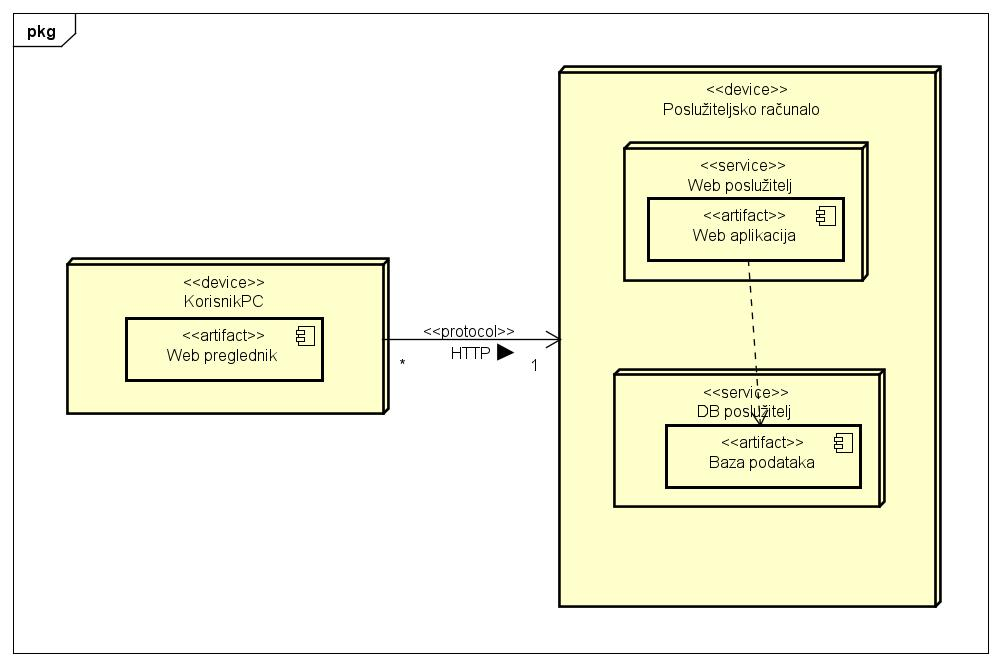
\includegraphics[scale=0.3]{slike/Dijagram razmjestaja}
				\centering
				\caption{Dijagram razmještaja}
				\label{fig:razmijestaja}
			\end{figure}

			\eject 
		
		\section{Upute za puštanje u pogon}
		
			\textbf{\textit{dio 2. revizije}}\\
		
			 \textit{U ovom poglavlju potrebno je dati upute za puštanje u pogon (engl. deployment) ostvarene aplikacije. Na primjer, za web aplikacije, opisati postupak kojim se od izvornog kôda dolazi do potpuno postavljene baze podataka i poslužitelja koji odgovara na upite korisnika. Za mobilnu aplikaciju, postupak kojim se aplikacija izgradi, te postavi na neku od trgovina. Za stolnu (engl. desktop) aplikaciju, postupak kojim se aplikacija instalira na računalo. Ukoliko mobilne i stolne aplikacije komuniciraju s poslužiteljem i/ili bazom podataka, opisati i postupak njihovog postavljanja. Pri izradi uputa preporučuje se \textbf{naglasiti korake instalacije uporabom natuknica} te koristiti što je više moguće \textbf{slike ekrana} (engl. screenshots) kako bi upute bile jasne i jednostavne za slijediti.}
			
			
			 \textit{Dovršenu aplikaciju potrebno je pokrenuti na javno dostupnom poslužitelju. Studentima se preporuča korištenje neke od sljedećih besplatnih usluga: \href{https://aws.amazon.com/}{Amazon AWS}, \href{https://azure.microsoft.com/en-us/}{Microsoft Azure} ili \href{https://www.heroku.com/}{Heroku}. Mobilne aplikacije trebaju biti objavljene na F-Droid, Google Play ili Amazon App trgovini.}

            {Kako se aplikacija sastoji od dva distinktivna dijela, backend-a i frontend-a, svaki dio funkcionira samo za sebe te se zasebno pušta u pogon.}

			\subsection{Backend}

                {Backend se sastoji od koda u obliku gradle projekta u rađenom u Spring boot okruženju. Kako Spring boot samostalno radi tablice i ažurira relacije u bazi podataka, potrebno je samo na poslužitelju na kojem će se nalaziti kompajliran pokrenut kod stvoriti bazu podataka s nazivom \textit{cdb}.}
                
                {Za početak je potrebno otvoriti virtualni stroj s ubuntu serverom na poslužitelju po izboru nakon čega je potrebno unesti sljedeće naredbe koristeći command prompt kako bi se ulogirali i postavili server:}

                \begin{packed_item}
        			\item {ssh root@ipv4AdresaServera}
        			\item {sudo apt update}
        			\item {sudo apt upgrade}
        			\item {sudo apt install fail2ban}
        			\item {sudo systemctl restart fail2ban.service}
        		\end{packed_item}

                {Sada kada je server postavljen, potrebno je instalirati postgresql i podignuti bazu naziva cdb:}

                \begin{packed_item}
        			\item {sudo apt-get install postgresql postgresql-contrib}
        			\item {sudo systemctl start postgresql.service}
        			\item {sudo systemctl enable postgresql.service}
        			\item {sudo -u postgres psql}
        			\item {\textbackslash password postgres}
        			\item {CREATE DATABASE cdb}
        			\item {\textbackslash c cdb}
        			\item {\textbackslash q}
        		\end{packed_item}

                {Nakon što je baza podataka na serveru stvorena, potrebno je kompajlirati kod za backend aplikacije te ga tako kompajliranog prebaciti na server. Sljedeće naredbe potrebno je izvršiti u matičnog folderu koda preuzetnog na vlastito računalo:}

                \begin{packed_item}
        			\item {cd Backend}
        			\item {gradle bootJar}
        			\item {scp build/libs/backend-0.0.1-SNAPSHOT.jar root@ipv4AdresaServera:/var/www}
        		\end{packed_item}

                {Nakon što je kompajlirani kod na serveru, potrebno je instalirati javu kako bi ga mogli pokrenuti:}

                \begin{packed_item}
        			\item {sudo apt install openjdk-17-jdk}
        		\end{packed_item}

                {Kako bi osigurali da aplikacija radi i kada na serveru ne postoji ulogirani korisnik, potrebno je kompajliran kod pokrenuti kao servis:}

                \begin{packed_item}
        			\item {cd /usr/lib/systemd/system}
        			\item {nano runSpringServer.service}
        			\item \textit{Sljedeći kod upiši u novootvoreni text editor:}
        			\item {[Unit]}
                    \item {Description=webserver Daemon}
                    \item {[Service]}
                    \item {ExecStart=/usr/bin/java -jar /var/www/backend-0.0.1-SNAPSHOT.jar}
                    \item {User=root}
                    \item {[Install]}
                    \item {WantedBy=multi-user.target}
        			\item \textit{Zatvori text editor koristeći kombinacije tipki CTRL+S pa CTRL+X.}
        			\item {sudo systemctl start runSpringServer.service}
        			\item {sudo systemctl enable runSpringServer.service}
        		\end{packed_item}

            \subsection{Frontend}

                {}
			
			\eject 